\documentclass[10pt, a4paper]{article}

\usepackage[paper=a4paper, left=1.5cm, right=1.5cm, bottom=1.5cm, top=3.5cm]{geometry}
\usepackage[utf8]{inputenc}
\usepackage[spanish]{babel}
\usepackage{caratula}
\usepackage{framed}
\usepackage{ulem}
\usepackage[pdftex]{graphicx}
\usepackage{float}
\usepackage{listings}
\usepackage{hyperref}


%Datos para la caratula
\materia{Teoría de Lenguajes}

\titulo{Trabajo Práctico}

\integrante{Ciraco Agustina}{630/06}{agusciraco@gmail.com}
\integrante{Heredia Mart\'in}{146/11}{martin.heredia@gmail.com}
\integrante{Tastzian Juan Manuel}{39/10}{jm@tast.com.ar}
\fecha{27 de Noviembre de 2014}


\begin{document}
	\maketitle
	\tableofcontents
	
	\newpage
	\section{Introducci\'on}
	\section{Introducción}

\clearpage

	
	\section{Cambios de la Reentrega}
	\begin{itemize}
\item Para mejorar la descripci\'on y entendimiento de algunas expresiones regulares que eran innecesariamente extensas, se decidi\'o modificar algunas expresiones regulares correspondientes a tokens, como así tambien se modificó la gram\'atica y su implementaci\'on. Anteriormente, había ciertos casos en que no se capturaban correctamente ciertas reglas. Por ejemplo la regla \textbf{ballon}, ya que el prefijo \textbf{ball} coincide con una primitiva, y era considerado como tal. \\
Ahora, la modificaci\'on realizada permite tomar un string completo $([a-zA-Z]+|\$|\_)$, como por ejemplo \texttt{ballon} y ver si se corresponde con una primitiva. En este caso no se corresponde por lo que puede ser nombre de una regla (y es considerado como un token \textbf{RULE\_NAME}).

\item Respecto al c\'odigo se realizaron arreglos para que funcione con los ejemplos de programa v\'alidos que se muestran en la presentaci\'on de este trabajo pr\'actico. Por ejemplo hab\'ia un problema con las definiciones de las rotaciones, que ahora se puede ver que funciona como se deseaba acorde a la presentaci\'on.
\\
Se modific\'o el c\'odigo que realiza la visualizaci\'on, ya que anteriormente ten\'ia problemas con la m\'axima profundidad.
\\
Tambi\'en se arregl\'o la forma de multiplicar las matrices en los \texttt{getters} de las clases creadas para la visualizaci\'on. La descripci\'on de las mismas se encuentra en la secci\'on de implementaci\'on.


\item Cambios en la gram\'atica: Se elimin\'o el no terminal \textbf{INITIAL\_AUXILIAR} y las producciones que lo utilizaban, se modificaron las expresiones regulares para algunos tokens y algunas producciones.

\end{itemize}


%~ Para emprolijar algunas expresiones regulares que qnos habian quedado innecesariamente extensas decidimos, modificar la gramatica asociando en keywords algunos tokens. Por ejemplo Ball Box  y void pasaron a ser keywords_tipo y las transformaciones pasaron a estar asociadas en un keywords_transformation.
%~ De esta manera la lista de tokens queda mas reducible y facil de leer, y lo mismo para sus respectivas expresiones regulares.
%~ En particular cambio mucho la definicion de regla, pues ahora toma todo un string de caracteres y luego verifica que sea un keyword.
%~ 
%~ Respecto al codigo hubo varios arreglos, pues por ejemplo las rotaciones estaban mal, luego, se refactorizo el c\'odigo del show, para un codigo mas reducible y facil de leer.
%~ la forma de multiplicar de las matrices en la clase de transformation en los geters 
%~ se arreglo el calculo de la profundidad.
%~ 
%~ Se saco el simbolo distinguido "initial_auxiliar" y las respectivas producciones que lo usaban, y esto se ve reflejado en el archivo yacc.py
%~ 
%~ Ahora el simbolo distinguido es initial
%~ 
%~ Cambiamos el nombre del token por uname para que se entienda que solo es un nombre

	
	%~ \newpage
	\section{Descripción de la Gramática}
	$G\ =\ <\ V_N\ ,\ V_T\ ,\ P\ ,\ INITIAL\_AUXILIAR\ >$\\

donde:\\
\begin{itemize}
%~ \item []$\mathbf{V_N}\ =\ \{ INITIAL\_AUXILIAR, INITIAL\_AUXILIAR, INITIAL,  LINE, RULE\_HEADER, DISY, rule, F, EXPR, TERM, FACTOR, \\

\item []$\mathbf{V_N}\ =\ \{ INITIAL\_AUXILIAR, INITIAL, LINE, DISY, RULE, F, EXPR, TERM, FACTOR, \\
CONJ, TRANSFORMATION, ELEM\_FACTOR \}$

\item []$\mathbf{V_T}\ =\  \{ NUM, RULE_NAME, EQUALS, DDOT, AND, ADD, SUB, MUL, DIV, OR, POW, LBRACKET, RBRACKET, LPAREN, RPAREN, LESS, GREATER, POINT, PRIMITIVE, TRANSFORMATION\}$
\item []$\mathbf{S}\ =\ S$
\item []$\mathbf{P}\ =\ Producciones$
\end{itemize}
\subsection{Conjunto de Tokens}

\begin{itemize}
 \item []$\mathbf{NUM}\ =\ r'\backslash d+(\backslash .\backslash d+)?'$
 \item []$\mathbf{RULE}\ =\ r'(x[a-zA-Z]+)|(y[a-zA-Z]+)|(z[a-zA-Z]+)|(r[a-wA-Z][a-zA-Z]*)|(s[a-wA-Z][a-zA-Z]*)|(t[a-wA-Z][a-zA-Z]*)|(c[aA-Z|c-fA-Z|h-qA-Z|s-zA-Z][a-zA-Z]*)|(d[a-zA-Z]+)|([a-b|e-q|u-w|A-Z][a-zA-Z]*)|\\x24'
$
 \item []$\mathbf{BALL}\ =\ r'ball'$
 \item []$\mathbf{BOX}\ =\ r'box'$
 \item []$\mathbf{VOID}\ =\ r'\_'$
 \item []$\mathbf{ROTATION}\ =\ r'r'$
 \item []$\mathbf{SCALE}\ =\ r's'$
 \item []$\mathbf{COLOR\_R}\ =\ r'c[\backslash s]*r'$
 \item []$\mathbf{COLOR\_G}\ =\ r'c[\backslash s]*g'$
 \item []$\mathbf{COLOR\_B}\ =\ r'c[\backslash s]*b'$
 \item []$\mathbf{TRANSLATION}\ =\ r't'$
 \item []$\mathbf{DEPTH}\ =\ r'd'$
 \item []$\mathbf{EQUALS}\ =\ r'='$
 \item []$\mathbf{DDOTE}\ =\ r':'$
 \item []$\mathbf{X}\ =\ r'x'$
 \item []$\mathbf{Y}\ =\ r'y'$
 \item []$\mathbf{Z}\ =\ r'z'$
 \item []$\mathbf{AND}\ =\ r'\&'$
 \item []$\mathbf{ADD}\ =\ r'\backslash +'$
 \item []$\mathbf{SUB}\ =\ r'-'$
 \item []$\mathbf{MUL}\ =\ r'\backslash *'$
 \item []$\mathbf{DIV}\ =\ r'/'$
 \item []$\mathbf{OR}\ =\ r'\backslash x7C'$
 \item []$\mathbf{POT}\ =\ r'\backslash x5E'$
 \item []$\mathbf{LBRACKET}\ =\ r'\backslash x5B'$
 \item []$\mathbf{RBRACKET}\ =\ r'\backslash x5D'$
 \item []$\mathbf{LPAREN}\ =\ r'\backslash x28'$
 \item []$\mathbf{RPAREN}\ =\ r'\backslash x29'$
 \item []$\mathbf{LESS}\ =\ r'\backslash x3C'$
 \item []$\mathbf{GREATER}\ =\ r'\backslash x3E'$
 \item []$\mathbf{POINT}\ =\ r'\backslash x2E'$
\end{itemize}


\noindent



\newpage
\subsection{Conjunto de Producciones}

\begin{enumerate}
\item $INITIAL\_AUXILIAR$ $\rightarrow$ $INITIAL$ \\
\item $INITIAL$   $\rightarrow$  $LINE$ $INITIAL$ \\
\item $INITIAL$   $\rightarrow$  $LINE$ \\
\item $LINE$   $\rightarrow$  $RULE$ $=$ $DISY$ \\
\item $LINE$   $\rightarrow$  $RULE$ $.$ $=$ $DISY$ \\

%~ // Para aritmetica
\item $EXPR$ $\rightarrow$ $TERM$ $ADD$ $EXPR$ \\
\item $EXPR$ $\rightarrow$ $TERM$ $SUB$ $EXPR$ \\
\item $EXPR$ $\rightarrow$ $TERM$ \\

\item $TERM$ $\rightarrow$ $FACTOR$ $MULT$ $TERM$\\
\item $TERM$ $\rightarrow$ $FACTOR$ $DIV$ $TERM$\\
\item $TERM$ $\rightarrow$ $FACTOR$\\

\item $FACTOR$ $\rightarrow$ $ADD$ $NUM$ \\
\item $FACTOR$ $\rightarrow$ $SUB$ $NUM$ \\
\item $FACTOR$ $\rightarrow$ $NUM$ \\
\item $FACTOR$ $\rightarrow$ $LBRACKET$ $EXPR$ $RBRACKET$\\

%~ // Desambiguacion de & y |

\item $DISY$   	$\rightarrow$  $CONJ$ \textbar $DISY$ \\
\item $DISY$   	$\rightarrow$  $CONJ$ \\

\item $CONJ$   	$\rightarrow$  $ELEM\_FACTOR$ \& $CONJ$ \\
\item $CONJ$   	$\rightarrow$  $ELEM\_FACTOR$ \\

\item $PRIM$	$\rightarrow$	$ball$ \textbar $box$ \textbar \_ \\
\item $ELEM\_FACTOR$   	$\rightarrow$  $<$ $DISY$ $>$ \\
\item $ELEM\_FACTOR$   	$\rightarrow$  [ $DISY$ ] \\
\item $ELEM\_FACTOR$ 	$\rightarrow$  $ELEM\_FACTOR$ T \\
\item $ELEM\_FACTOR$ 	$\rightarrow$  $RULE$ \\
\item $ELEM\_FACTOR$   	$\rightarrow$  $ELEM\_FACTOR$ $\widehat{}$ $EXPR$\\


\item $ELEM\_FACTOR$   	$\rightarrow$  $BALL$\\
\item $ELEM\_FACTOR$   	$\rightarrow$  $BOX$\\
\item $ELEM\_FACTOR$   	$\rightarrow$  $\_$\\


\item $TRANSFORMATION$  $\rightarrow$   :$rx$ $NUM$ \textbar :$ry$ $NUM$ \textbar :$rz$ $NUM$ \\
\item $TRANSFORMATION$	$\rightarrow$	:$tx$ $NUM$ \textbar :$ty$ $NUM$ \textbar :$tz$ $NUM$ \\
\item $TRANSFORMATION$	$\rightarrow$	:$sx$ $NUM$ \textbar :$sy$ $NUM$ \textbar :$sz$ $NUM$ \textbar :$s$ $NUM$ \\
\item $TRANSFORMATION$ 	$\rightarrow$	:$cr$ $NUM$ \textbar :$cg$ $NUM$ \textbar :$cb$ $NUM$ \\
\item $TRANSFORMATION$	$\rightarrow$	:$d$  $NUM$ \\



\end{enumerate}

\noindent

	
	\newpage
	\section{Discusión de la Gramática}
	\subsection{Decisiones tomadas}

Al generar la gram\'atica detallada anteriormente se debieron tomar las siguientes decisiones:

\begin{itemize}
\item[•] Se decidi\'o definir los tokens \textbf{COLOR\_R}, \textbf{COLOR\_G} y  \textbf{COLOR\_B}, con la expresión regular incluyendo la letra del color, para evitar ambiguedades tales como, por ejemplo el $mathbf{'r'}$ pueda ser considerada describiendo una rotación o el color red.

\item[•] Para los caracteres que podr\'ian llegar a tener conflicto, como por ejemplo los par\'entesis o los corchetes, se decidi\'o utilizar el c\'odigo de dicho caracter en \textbf{UNICODE}, ya que los mismos son considerados caracteres especiales.

\end{itemize}

\subsection{Comentarios sobre algunos tokens}
\begin{itemize}
\item[•] $\mathbf{RULE}$: Este token se decidi\'o definir con esa uni\'on de expresiones regulares porque, de no ser de esa manera, pod\'ia tener conflictos con otras definiciones de tokens, como por ej\'emplo las transformaciones o las rotaciones, pues una regla podr\'ia consistir de un \" r = \". M\'as adelante se detalla un problema espec\'ifico que se encontr\'o al momento de implementarlo con \textbf{PLY}\footnote{Python Lex Yacc}. 

\item[•] $\mathbf{OR}\ =\ r'\backslash x7C'$ El s\'imbolo $'\backslash x7C'$ hace referencia al caracter $' \textbar '$ en unicode.
%~ \item[•] $\mathbf{POT}\ =\ r'\backslash x5E'$ El s\'imbolo $'\backslash x5E'$ hace referencia al caracter $' \textasciicircum '$ en unicode.
\item[•] $\mathbf{POT}\ =\ r'\backslash x5E'$ El s\'imbolo $'\backslash x5E'$ hace referencia al caracter $' \widehat{} '$ en unicode.
\item[•] $\mathbf{LBRACKET}\ =\ r'\backslash x5B'$ En este caso, la referencia al s\'imbolo $'['$ est\'a dada por $'\backslash x5B'$. 
\item[•] $\mathbf{RBRACKET}\ =\ r'\backslash x5D'$ Similar al caso anterior, el s\'imbolo $']'$ es representado por $'\backslash x5D'$.
\item[•] $\mathbf{LPAREN}\ =\ r'\backslash x28'$ En este token el s\'imbolo $'\backslash x28'$ referencia al s\'imbolo $'('$. 
\item[•] $\mathbf{RPAREN}\ =\ r'\backslash x29'$ Similar al anterior el s\'imbolo $')'$ es referenciado por $'\backslash x29'$. 
\item[•] $\mathbf{LESS}\ =\ r'\backslash x3C'$ En este caso, el s\'imbolo $'\backslash x3C'$ en unicode esta referenciando al s\'imbolo $'<'$. 
\item[•] $\mathbf{GREATER}\ =\ r'\backslash x3E'$ Similar al caso anterior, el s\'imbolo $'>'$, es referenciado por $'\backslash x3E'$.
\item[•] $\mathbf{POINT}\ =\ r'\backslash x2E'$ En este caso, el s\'imbolo $'\backslash x2E'$ hace referencia al s\'imbolo $'.'$

\end{itemize}

	
	\newpage
	\section{Implementaci\'on}
	\subsection{Herramientas utilizadas}

Para la implemetaci\'on del analizador l\'exico y sint\'actico de la gram\'atica propuesta, se decidi\'o utilizar las herramientas propuestas por la c\'atedra. Las mismas son:

\begin{itemize}

\item [] \textbf{PLY}: \href{http://www.dabeaz.com/ply/}{Python Lex Yacc} es una implementaci\'on de las herramientas \textbf{Lex} \textbf{Yacc}
%\href{http://www.wikibooks.org}{Lex} y \href{http://www.wikibooks.org}{Yacc} en pyhton.

\item [] \textbf{VPython}: \href{http://vpython.org/index.html}{Visual Python} es una herramienta para programaci\'on gr\'afica.

\end{itemize}

\subsection{Decisiones para la implementaci\'on}

Para la correcta implemetaci\'on del analizador l\'exico se tuvo en cuenta la forma en que \href{http://www.dabeaz.com/ply/ply.html#ply_nn3}{PLex} evalua el orden de los tokens, ya que toma la expresi\'on regular de mayor longitud, y luego las dem\'as en orden aleatorio. Esto tra\'ia problemas al analizar ciertas experesiones, tales como \textbf{ball}, ya que la misma estaba siendo considerada un token \textbf{Rule} porque primero estaba evaluando esa expresi\'on regular, y en particular el lenguaje aceptado por la dicha expresi\'on acepta la cadena $'ball'$. Por ello se decidi\'o forzar a el orden en que eval\'ue ciertas reglas.
\\
\\
Luego, para poder implementar comentarios, y que se pueda ignorar el contenido, se utiliz\'o la notaci\'on de \textbf{t\_ignore} seguido de un nombre declarativo para lo que se desee ignorar, por ej\'emplo en este caso, \textbf{t\_ignore\_comment}.
\\
\\
En el caso de analizador sint\'actico se decidi\'o utilizar un diccionario para guardar las transformaciones de un elemento, en la primer posici\'on del par\'ametro \textbf{p}.
\\
\\
Al momento de poder decir que una expresi\'on es v\'alida, es decir, que pudo pasar por el analizador l\'exico, luego por el sint\'actico y no produjo error, debemos poder ejecutarla correctamente. Para esto se tuvo que tomar otra decisi\'on, ya que la utilizaci\'on de la herramienta visual python por si sola no alcanzaba para los objetivos de este trabajo pr\'actico. Esto se debe a que al momento de mostrar esta expresi\'on, queremos contemplar ciertas probabilidades y relaciones con el \textbf{ \& } u el \textbf{ \textbar } que la herramienta por si sola no contempla. 
Para ello, se implemento una jerarqu\'ia de clases para poder mostrar acorde a los requerimientos de este trabajo pr\'actico.


\subsection{C\'odigo}

El c\'odigo se dividi\'o en 3 archivos principales y uno de auxiliares:
\begin{itemize}
\item [] \textbf{lexer.py:} Este archivo contiene la implementaci\'on del analizador l\'exico. Para dicha implementaci\'on se defini\'o la lista de tokens, presentada en la secci\'on de descripci\'on de la gram\'atica, y luego las expresiones regulares para cada token, incluyendo las expresiones de lo que se desea ignorar, como por ejemplo los comentarios. Luego, la llamada a la herramienta a \textbf{lex.lex()} para generar el analizador l\'exico de la gram\'atica propuesta.

\item [] \textbf{yacc.py:} En este archivo se encuentra la implementaci\'on del analizador sint\'actico, que incluye las definiciones de las producciones definidas en la secci\'on de descripci\'on de la gram\'atica. Seg\'un a qu\'e expresi\'on corresponde se define lo que se desea guardar en el diccionario. Por \'ultmo, la llamada a la herramienta \textbf{yacc.yacc()} para generar el analizador sint\'actico. Cabe destacar que para generar el analizador sint\'actico se requiere de la lista de tokens y de analizador l\'exico, por lo que ambos se incluyen del archivo anterior.

\item [] \textbf{definition.py:} Este archivo contiene la implementaci\'on de los procedimientos requeridos para la visualizaci\'on de los resultados, el mismo se implement\'o en una jerarqu\'ia de clases para realizar la visualizaci\'on de los objetosacorde a las probabilidades deseadas, junto con las diferentes formas de visualizar. La clase padre es \textbf{Definition} que contiene una funci\'on para cada forma posible de mostrar objetos. 

\item [] \textbf{functions.py} Este archivo contiene unas funciones auxiliares.
\end{itemize}

A continuaci\'on se presenta el c\'odigo contenido en cada archivo.

\newpage
\subsubsection{lexer.py}

\lstinputlisting[language=Python,breaklines=true]{../lexer.py}

\newpage
\subsubsection{yacc.py}

\lstinputlisting[language=Python,breaklines=true]{../yacc.py}

\newpage
\subsubsection{definition.py}

\lstinputlisting[language=Python,breaklines=true]{../definition.py}


\newpage
\subsubsection{functions.py}

\lstinputlisting[language=Python,breaklines=true]{../functions.py}


\newpage
\subsubsection{Modo de uso}


	
	\newpage
	\section{Ej\'emplos de \'arboles de derivaci\'on con entradas correctas}
	En esta secci\'on se presentan algunos \'arboles de derivaci\'on de cadenas v\'alidas para la gram\'atica presentada.\\

\subsection{Ejemplo 1 - Aritm\'etico}
El siguiente ej\'emplo corresponde a la cadena:\\
$+N / (N-N*N*-N)$
Lo interesante de esta cadena es ver que no genera ambiguedades con el uso de los signos para los n\'umeros.
\begin{figure}[!h]
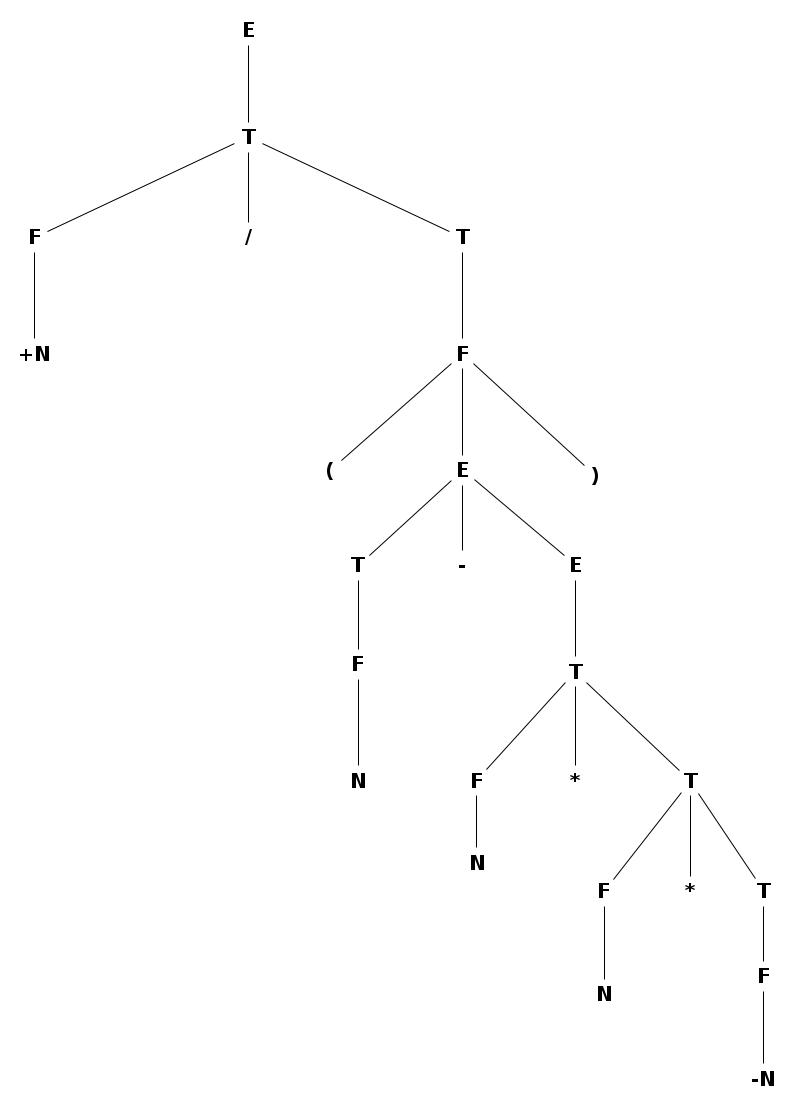
\includegraphics[scale=0.40]{arboles_derivacion/ejemplo1.jpg}
\end{figure}
\subsection{Ejemplo 2 - Aritm\'etico}
El ej\'emplo 2 se corresponde a la cadena:
$N*N+N*N$
\centerline{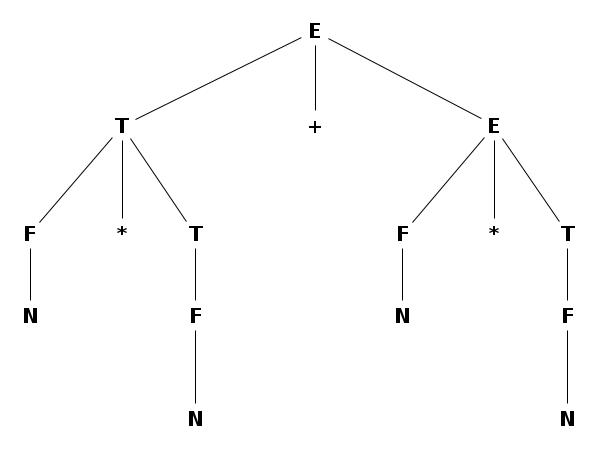
\includegraphics[scale=0.40]{arboles_derivacion/ejemplo2.jpg}}

\subsection{Ejemplo 3 - Programa v\'alido}
%cube
\centerline{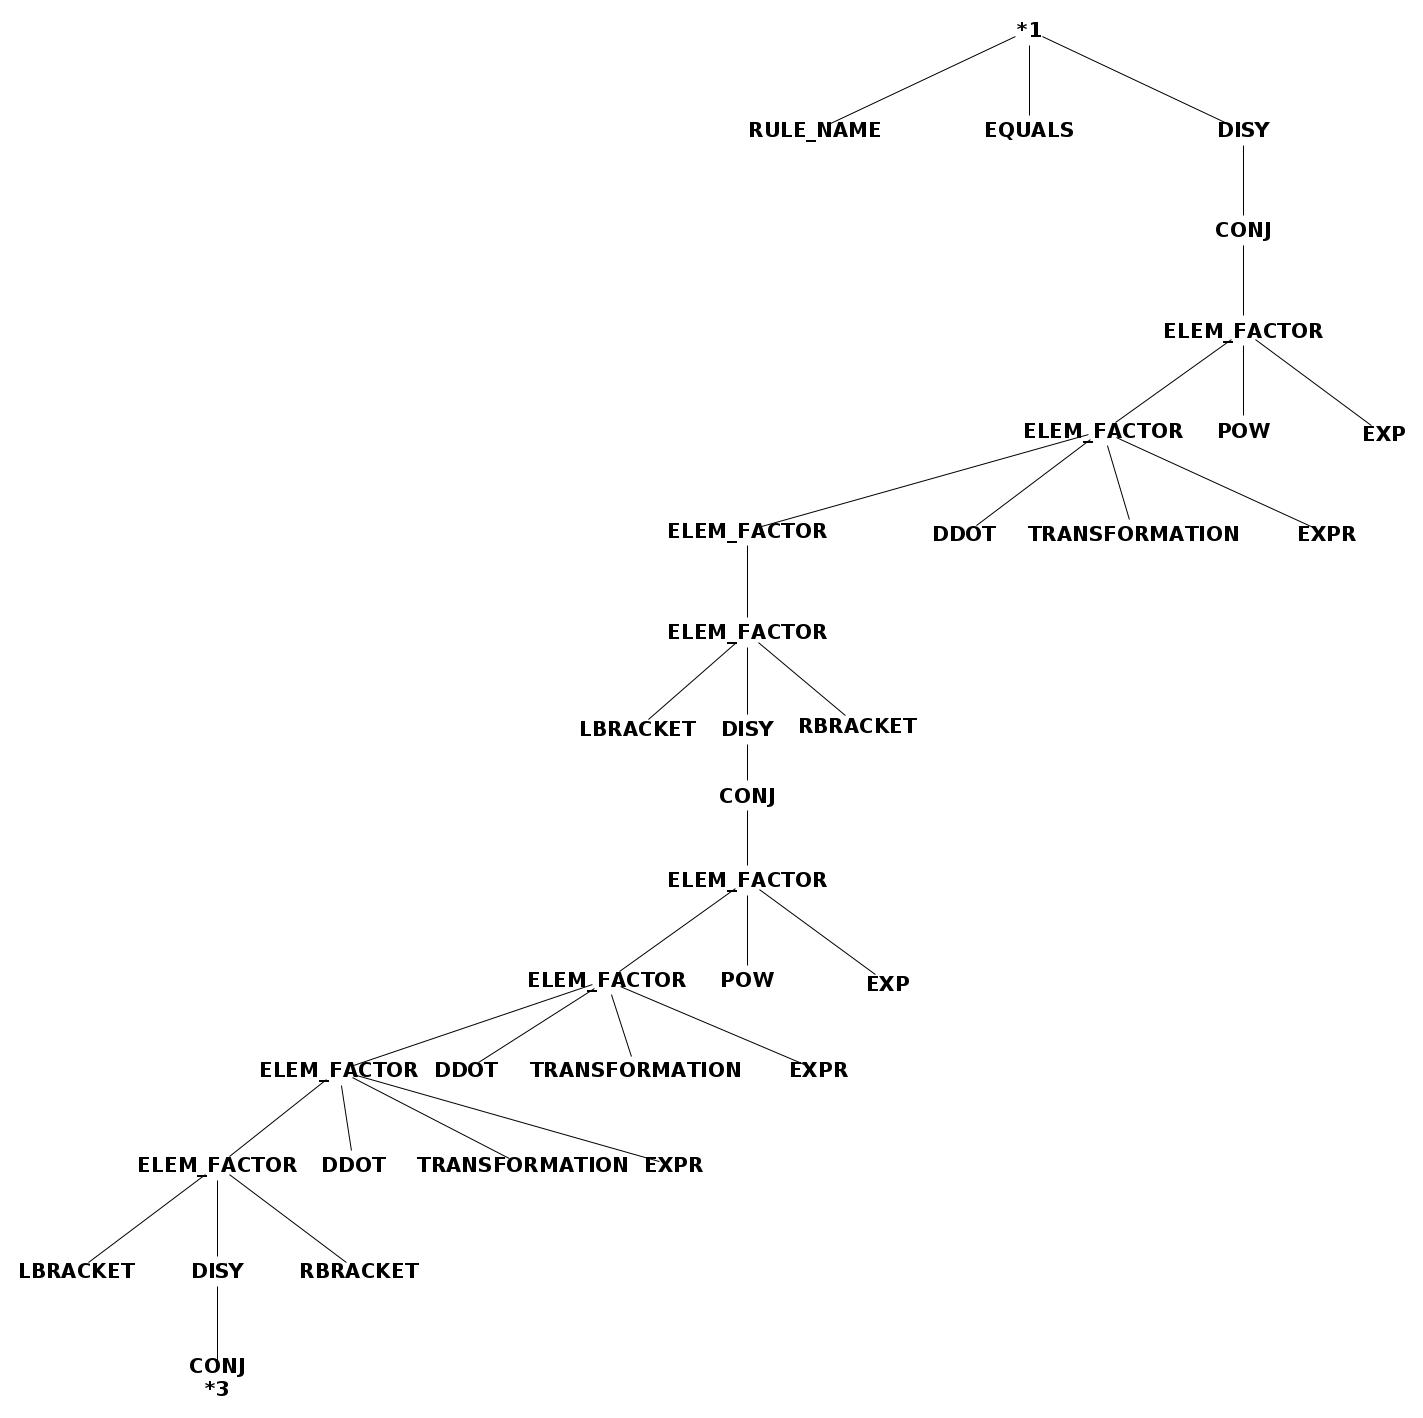
\includegraphics[scale=0.40]{arboles_derivacion/cube1.jpg}}

	
	
	\newpage
	\section{Ej\'emplos de programas}
	En esta secci\'on se presentan algunos ej\'emplos de programas con el resultado correspondiente.

\subsection{Programas v\'alidos}

El siguiente ejemplo, es un ejemplo que se llego a correr para la primer entrega de este trabajo, por lo que es un buen ejemplo para ver la evoluci\'on del c\'odigo. \\
Primero se va a mostrar el ejemplo del programa que se va a ejecutar, luego el resultado del c\'odigo de la primer entrega, y despu\'es el resultado correspondiente al c\'odigo presentado en esta entrega.\\
Para ver la diferencia de forma m\'as clara la im\'agen de fondo negro es la presentada anteriormente, y de fondo blanca es la actual.\\

\lstinputlisting[breaklines=true]{../Ejemplos/eg04.peg}


\centerline{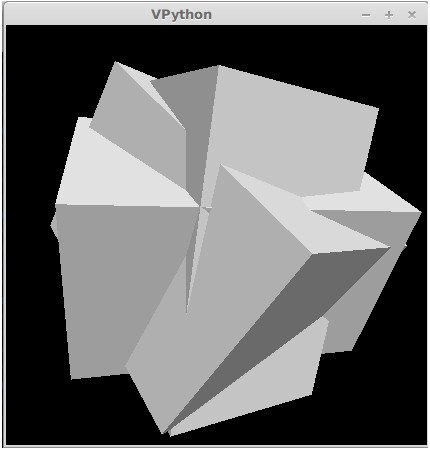
\includegraphics[scale=0.40]{../imagenes/eg04.jpg}}


\centerline{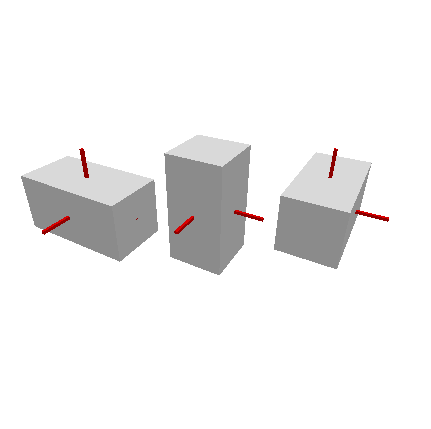
\includegraphics[scale=0.40]{../imagenes/eg04_nuevo.png}}


El ejemplo que se presenta a continuaci\'on, al igual que el anterior, se ejecut\'o con el c\'odigo de la entrega anterior y con el presentado en esta entrega. Por lo que tambi\'en se puede observar la diferencia entre ambos resultados.\\
Los mismos se presentan en el mismo orden correspondiente al ejemplo anterior.\\

\lstinputlisting[breaklines=true]{../Ejemplos/eg11.peg}


\centerline{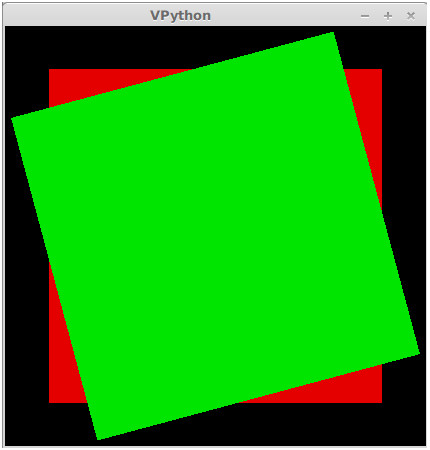
\includegraphics[scale=0.40]{../imagenes/eg11.jpg}}


\centerline{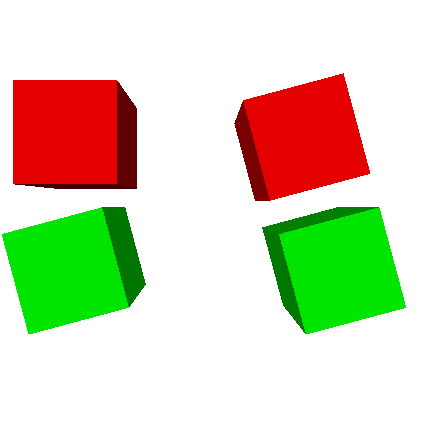
\includegraphics[scale=0.40]{../imagenes/eg11_nuevo.png}}

\newpage
Los siguientes ejemplos fueron ejecutados con el c\'odigo de esta entrega.\\
\lstinputlisting[breaklines=true]{../Ejemplos/eg22.peg}

\centerline{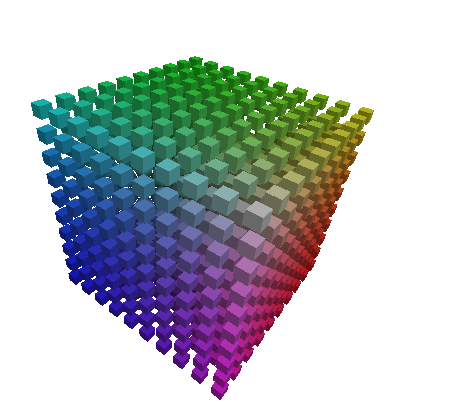
\includegraphics[scale=0.40]{../imagenes/eg22.png}}


\lstinputlisting[breaklines=true]{../Ejemplos/eg23.peg}

\centerline{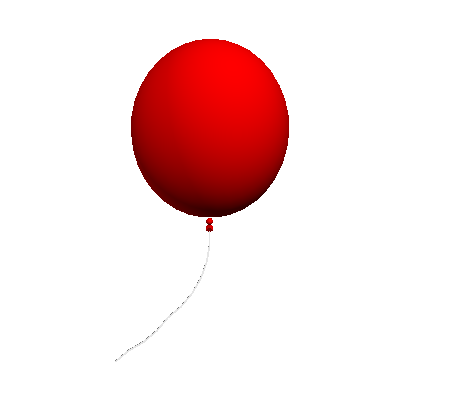
\includegraphics[scale=0.40]{../imagenes/eg23.png}}



\lstinputlisting[breaklines=true]{../Ejemplos/eg24.peg}

\centerline{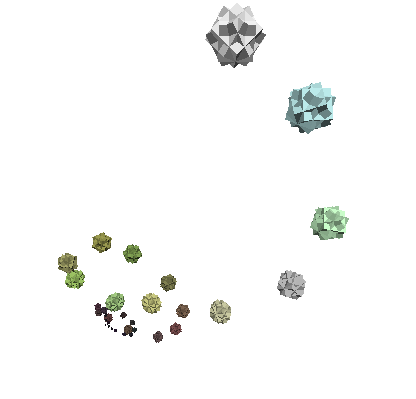
\includegraphics[scale=0.40]{../imagenes/eg24.png}}


\lstinputlisting[breaklines=true]{../Ejemplos/eg25.peg}

\centerline{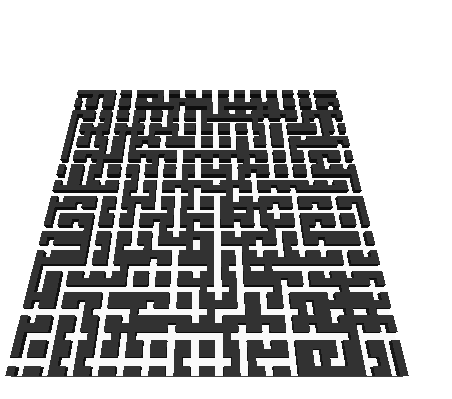
\includegraphics[scale=0.40]{../imagenes/eg25.png}}


\lstinputlisting[breaklines=true]{../Ejemplos/eg26.peg}

\centerline{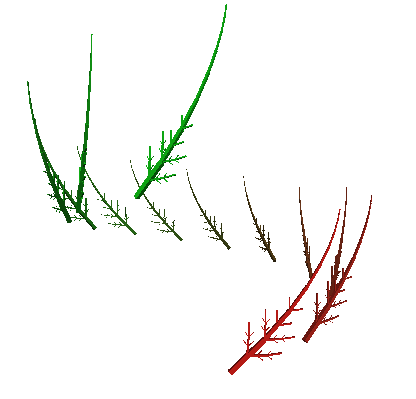
\includegraphics[scale=0.40]{../imagenes/eg26.png}}


\lstinputlisting[breaklines=true]{../Ejemplos/eg27.peg}

\centerline{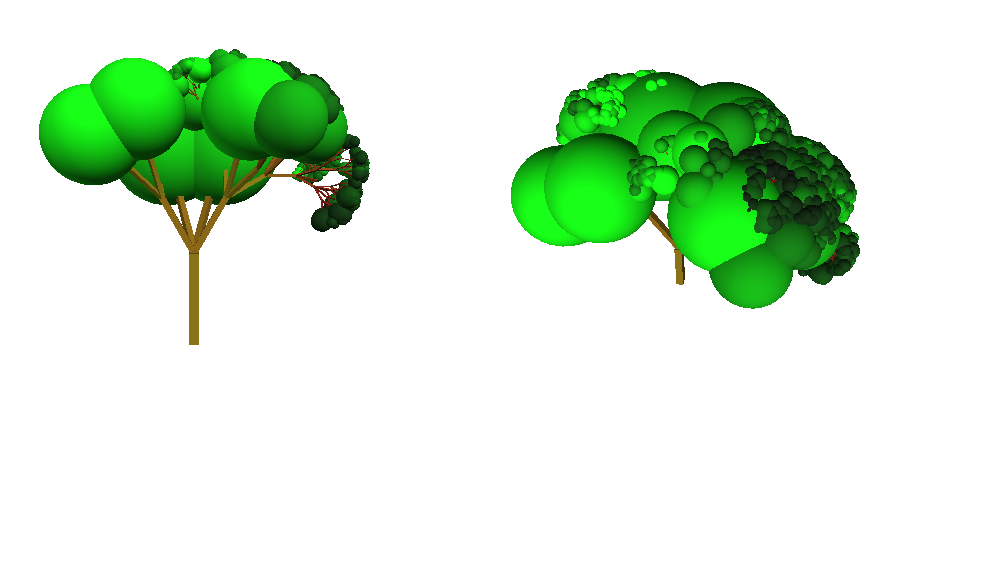
\includegraphics[scale=0.40]{../imagenes/eg27.png}}


\lstinputlisting[breaklines=true]{../Ejemplos/cara.peg}

\centerline{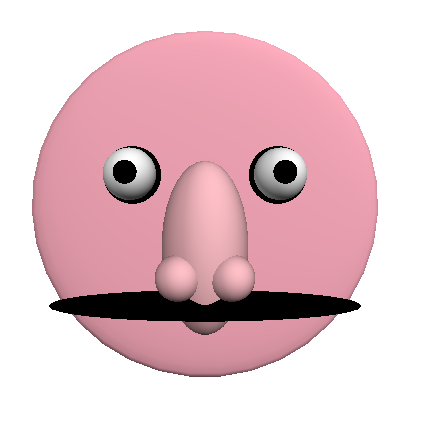
\includegraphics[scale=0.40]{../imagenes/cara.png}}

\newpage

\subsection{Programas inv\'alidos}

\lstinputlisting[breaklines=true]{../Ejemplos/eg22invalid.peg}

\centerline{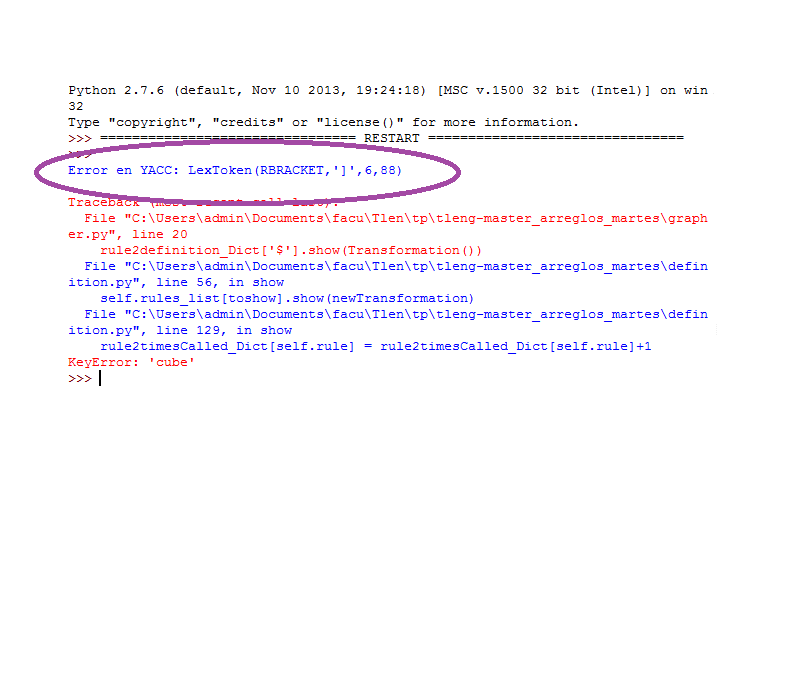
\includegraphics[scale=0.70]{../imagenes/eg22invalid.png}}

\lstinputlisting[breaklines=true]{../Ejemplos/eg22invalid2.peg}

\centerline{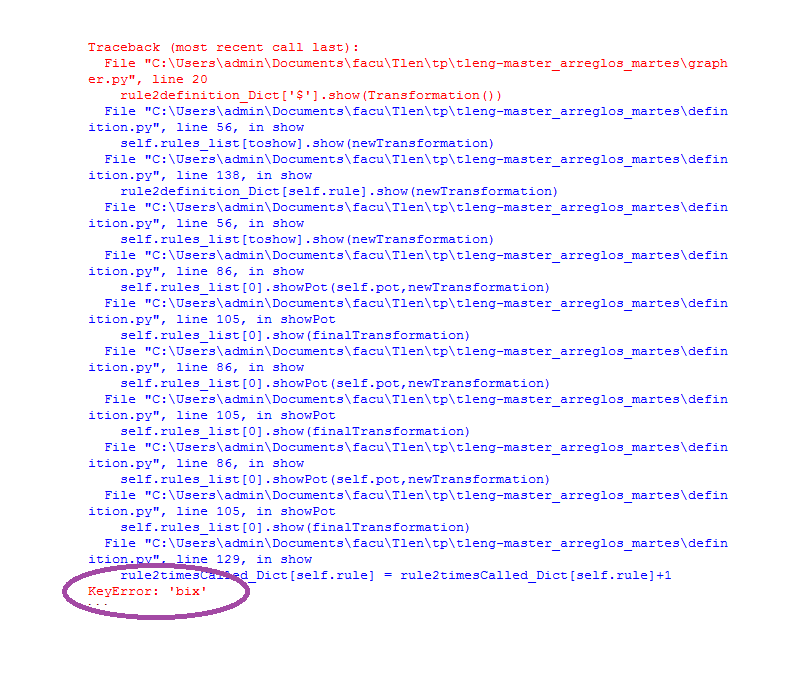
\includegraphics[scale=0.70]{../imagenes/eg22invalid2.png}}

\lstinputlisting[breaklines=true]{../Ejemplos/carainvalid.peg}

\centerline{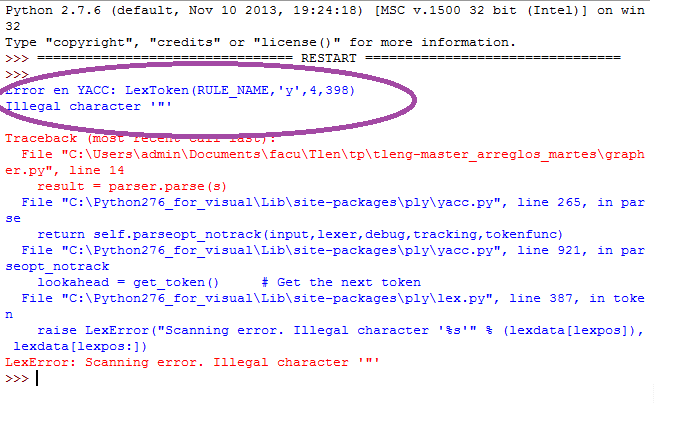
\includegraphics[scale=0.70]{../imagenes/carainvalid.png}}
	
	
\end{document}
